\documentclass[10pt,twocolumn]{article}

\usepackage[margin=0.75in]{geometry}
\usepackage{times}
\usepackage{amsmath,amssymb,amsthm}
\usepackage{booktabs}
\usepackage{graphicx}
\usepackage{hyperref}
\usepackage{xcolor}
\usepackage{microtype}
\usepackage{enumitem}

\newtheorem{theorem}{Theorem}
\newtheorem{lemma}{Lemma}
\newtheorem{definition}{Definition}
\newtheorem{proposition}{Proposition}

\newcommand{\F}{\mathbb{F}}
\newcommand{\Fp}{\mathbb{F}_p}
\newcommand{\Fptwo}{\mathbb{F}_{p^2}}
\newcommand{\eq}{\widetilde{\mathrm{eq}}}
\newcommand{\Com}{\mathrm{Com}}
\newcommand{\Tthink}{T_{\text{think}}}
\newcommand{\zkmoe}{\textsc{zkMoE-Reason}}

\title{\textbf{Cost Accounting for Verifiable Sparse Mixture-of-Experts Inference: A Prototype Study of Expert-Table Projection and Threshold Top-$k$ Proofs}}

\author{Nissan Pow \\ Orchestral Labs}

\date{}

\begin{document}
\maketitle

\begin{abstract}
Sparse Mixture-of-Experts (MoE) layers store $N$ expert matrices but apply only $k \ll N$ per token, so a verifiable-inference system that proves all $N$ experts wastes work. We study a prototype that proves only the $k$ active expert matrix--vector products with a sumcheck, then ties the resulting random evaluation point to a committed expert table by projecting the table at that point and opening a Brakedown-style polynomial commitment. We also implement and count constraints for a threshold-witness top-$k$ relation. \textbf{This manuscript retracts the claims of an earlier version}: the prototype does \emph{not} hide the routing (the opened indicator evaluations determine the selected indices), the table projection costs $\Theta(Nd^2)$ field operations, there is no soundness theorem for chain-of-thought folding (removed), and the router and expert-lookup sub-protocols are not composed into one proof. What remains is a measured cost study on one ARM CPU against a baseline we implemented ourselves (one sumcheck per expert). Over $d \in \{256,512,1024\}$ and $N \le 128$ with $k=2$ the prototype proves a layer $1.5$--$13.1\times$ faster than the dense baseline, with the gap shrinking as $d$ grows because the projection scan becomes the bottleneck ($2.8\times$ at $d=1024$). The threshold top-$k$ relation needs $3.1$--$18.7\times$ fewer constraints than a bitonic sorting network for $N \in [8,256]$. The succinct commitment-opening verifier is flat at $19$--$29$\,ms while a raw-table verifier grows from $20$ to $198$\,ms for $N$ from 4 to 128 at $d=256$. Code and raw results are public.
\end{abstract}

\section{Introduction}
Zero-knowledge machine learning (zkML) systems prove that an output was computed by a committed model~\cite{kang2022scaling,chen2024zkml,sun2024zkllm}. They treat the model as a static dense graph. In an MoE layer the router selects $k$ of $N$ experts per token, so proving all $N$ matrix products and masking the unselected ones costs $\Theta(Nd^2)$ ZK sumcheck work for a computation that needs $\Theta(kd^2)$.

This paper is a prototype study and states its limits up front.
\begin{itemize}[leftmargin=*,itemsep=2pt]
    \item \textbf{What we measure.} A pipeline that runs a blinded sumcheck over only the $k$ active experts, projects the committed expert table at the sumcheck's random point, and checks the projected value through a polynomial-commitment opening (Section~\ref{sec:lookup}); and a threshold-witness top-$k$ relation with an explicit constraint count (Section~\ref{sec:router}).
    \item \textbf{What we do not claim.} Routing privacy; sublinear prover cost in $N$; soundness for hidden-reasoning (chain-of-thought) folding; a single composed proof of MoE inference; novelty of range-based top-$k$ proofs (Section~\ref{sec:related}).
\end{itemize}
Section~\ref{sec:limits} lists the gaps in full.

\section{Related Work}
\label{sec:related}
\paragraph{Dense and MoE zkML.} \textsc{zkLLM}~\cite{sun2024zkllm} and \textsc{EZKL}/zkML~\cite{chen2024zkml} prove dense transformers. ZK-DeepSeek~\cite{wang2025zkdeepseek} builds a PLONKish proof of DeepSeek-V3 inference, which contains MoE layers and a sorting-based top-$k$ check. It is the closest prior system and it is a full-model construction, which our prototype is not; we did not run it and make no performance comparison.
\paragraph{Top-$k$ proofs.} VERIF~\cite{zhang2026verif} proves top-$t$ selection with a permutation-free, limb-decomposed range relation. Our threshold-witness relation (Section~\ref{sec:router}) is the same idea in the MoE setting, so we present it as an application and constraint count, not a new technique.
\paragraph{Lookups and folding.} \textsc{Lasso}~\cite{setty2024unlocking} and \textsc{LogUp}~\cite{habock2022logup} prove table lookups; \textsc{Nova}~\cite{kothapalli2022nova} and \textsc{HyperNova}~\cite{kothapalli2024hypernova} fold repeated computations. We use a transparent Brakedown-style commitment~\cite{golovnev2023brakedown}.

\section{Setting and Notation}
Let $p = 2^{61}-1$ and $\F_{p^2} = \Fp[u]/(u^2+1)$ (Fiat--Shamir challenges are drawn there). For a table $f:\{0,1\}^v\to\Fp$ write $\widetilde f(x)=\sum_b f(b)\,\eq(b,x)$ for its multilinear extension. The committed model contains expert matrices $E_0,\dots,E_{N-1}\in\Fp^{d\times d}$ packed into one polynomial $\widetilde E(j,r,c)$ and committed once with $\Com_{\text{PCS}}(E)$. For activation $h\in\Fp^d$ and selected indices $s_1,\dots,s_k$ the prover claims $y_i=E_{s_i}h$.

\section{Expert-Table Projection Pipeline}
\label{sec:lookup}
\begin{enumerate}[leftmargin=*,itemsep=2pt]
    \item \textbf{Active-only matmul sumcheck, $O(kd^2)$.} A blinded, batched sumcheck (Chiesa--Forbes--Spooner-style masking~\cite{chiesa2017zero}) proves $\sum_i\alpha_i\widetilde{y_i}(r^*)=\sum_c(\sum_i\alpha_i\widetilde{M_i}(r^*,c))\widetilde h(c)$ and ends at a random point $(r^*,c^*)$ with claims $v_i=\widetilde{M_i}(r^*,c^*)$.
    \item \textbf{Table projection, $\Theta(Nd^2)$.} The prover computes $e_j=\widetilde E(j,r^*,c^*)$ for \emph{all} $j$, which reads every expert entry once. This is one fused linear scan (a C99 \texttt{uint128} kernel in the artifact), not $N$ sumchecks, but it is linear in $Nd^2$. The verifier never computes $e$; the vector $e$ is prover-supplied and is only ever checked at one point through the opening in step 4.
    \item \textbf{Indicator sumcheck, $O(N)$.} For each $i$ the prover commits a one-hot vector $u^{(i)}$, proves booleanity and $\sum_ju^{(i)}_j=1$, and proves $\sum_j(\sum_i\lambda_iu^{(i)}_j)e_j=\sum_i\lambda_iv_i$ by a $\log N$-round sumcheck ending at a point $j^*$.
    \item \textbf{Commitment openings, $O(\sqrt{Nd^2})$.} The prover opens $\widetilde E(j^*,r^*,c^*)$ against $\Com_{\text{PCS}}(E)$ and each $\widetilde{u^{(i)}}(j^*)$ against its commitment.
\end{enumerate}

\paragraph{Claim (soundness only).} Assume a binding commitment, a sound tensor-code opening with error $\epsilon_{\text{PCS}}$, and the random-oracle model. If some $y_i\neq E_{s_i}h$, or if $M_i$ is not an expert in the committed table, the verifier accepts with probability at most $(2\log d+2\log N+2\log(kN))/|\Fptwo|+\epsilon_{\text{PCS}}$ plus negligible terms (Schwartz--Zippel on the matmul reduction, the booleanity and lookup sumchecks, and the opening). We do not claim zero knowledge.

\paragraph{Routing is not hidden.} In step 4 the opened value $\widetilde{u^{(i)}}(j^*)=\eq(s_i,j^*)$ for a fresh random $j^*$ is a deterministic function of $s_i$; any verifier can test the $N$ candidate indices and recover $s_i$ with overwhelming probability. Hiding it needs a zero-knowledge opening (for example a masked commitment with a simulator for every opened value), which this prototype lacks. A consequence worth stating: if routing is public, steps 3--4 are unnecessary, since the verifier can open $\widetilde E(s_i,r^*,c^*)$ directly. The indicator machinery only matters for the hiding variant, which is not achieved here.

\section{Threshold Top-$k$ Relation}
\label{sec:router}
Given quantized router logits $g\in[0,2^B)^N$, set $g'_j=g_jN+(N-1-j)$, which makes all $g'_j$ distinct. The prover supplies a mask $m\in\{0,1\}^N$ with $\sum_jm_j=k$ and a threshold $\tau$, and the margins $\delta_j=m_j(g'_j-\tau)+(1-m_j)(\tau-1-g'_j)$ must lie in $[0,2^{B+\lceil\log_2N\rceil})$ via bit decomposition.

\begin{proposition}
\label{prop:router}
$m$ selects the top-$k$ indices of $g'$ if and only if there is $\tau$ with every $\delta_j\ge 0$ (and $<2^{B+\lceil\log_2N\rceil}$). The relation has $O(NB_{\text{eff}})$ constraints, $B_{\text{eff}}=B+\lceil\log_2N\rceil$.
\end{proposition}
\begin{proof}
If all $\delta_j\ge0$, every selected $g'_j\ge\tau$ and every unselected $g'_j\le\tau-1$; with $\sum m_j=k$ and distinct values the selected set is exactly the $k$ largest. Conversely take $\tau=\min_{m_j=1}g'_j$; then $0\le\delta_j<N2^B$.
\end{proof}
This proves a statement about the relation only. We do not give a zero-knowledge proof for hiding $m$ and $\tau$, and the mask $m$ is not constrained to equal the indicators $u^{(i)}$ of Section~\ref{sec:lookup} (see Section~\ref{sec:limits}).

\section{Evaluation}
\label{sec:eval}
\paragraph{Setup.} One aarch64 machine, 14 cores at up to 2.6\,GHz, Python 3.10+ with NumPy 1.26 and a C99 Mersenne-61 kernel, single process. Each timing is the median of three runs after one warm-up run. Weights are random integers in $[0,128)$; the numbers say nothing about trained models. Timings exclude the one-time commitment of the expert table. The proofs are produced and checked by our research code, not an audited library.

\paragraph{Baseline.} ``Dense'' is our own implementation of the dense-masked approach: for every one of the $N$ experts, compute $y_j=E_jh$, commit it and run the same blinded sumcheck. It is a straightforward baseline, not \textsc{zkLLM} itself, and we did not tune it beyond sharing the sumcheck code. An earlier version also reported an extrapolated ``naive element-wise lookup'' baseline; we removed it because it was extrapolated from 128 sampled entries rather than measured.

\subsection{Sparsity scaling ($k=2$)}
\begin{figure}[t]
    \centering
    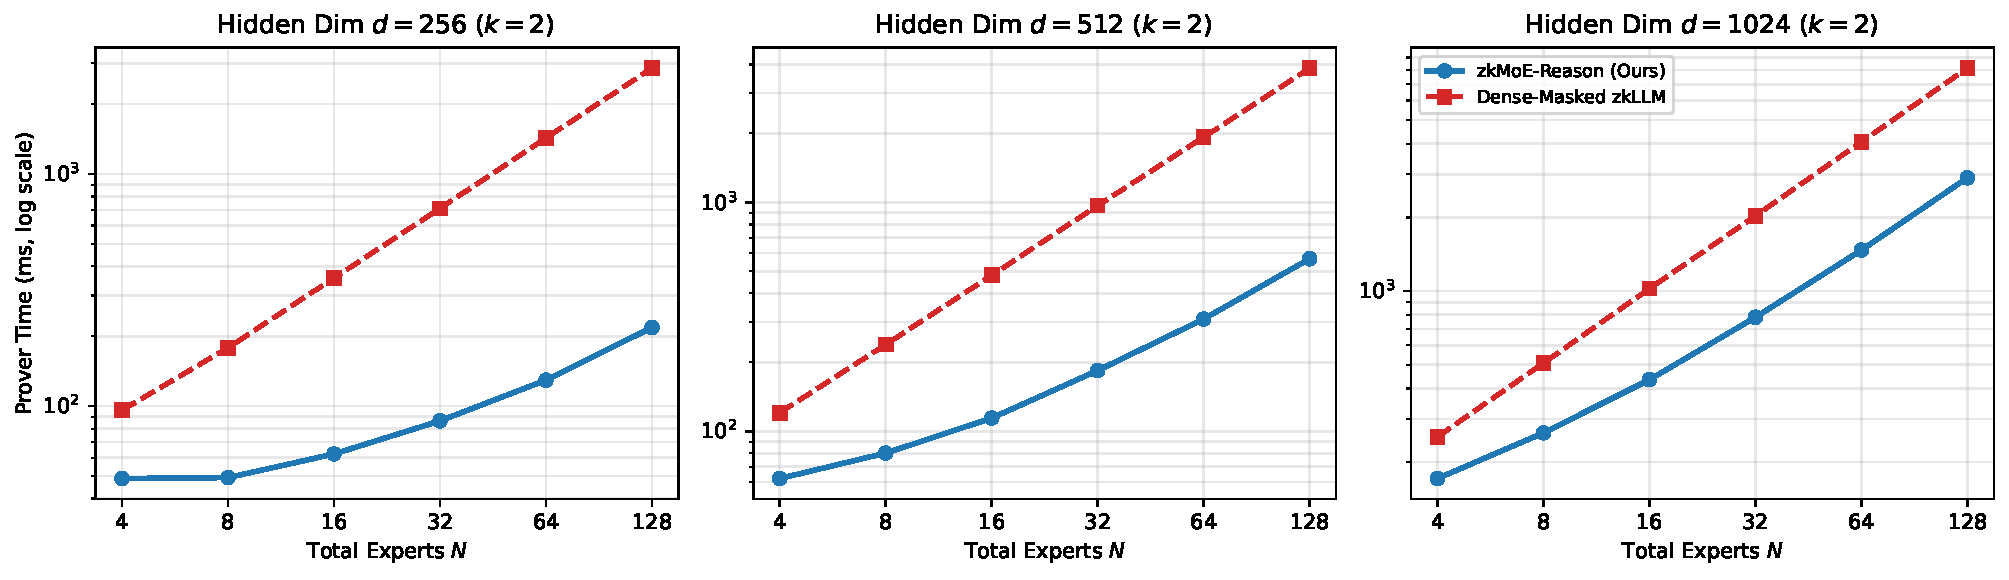
\includegraphics[width=\linewidth]{../results/exp1_sparsity_scaling.pdf}
    \caption{Prover time versus $N$ for $d\in\{256,512,1024\}$, $k=2$ (median of 3).}
    \label{fig:exp1}
\end{figure}
\begin{table}[t]
\centering
\small
\caption{Prover time (ms), median of 3 runs, $k=2$.}
\label{tab:exp1}
\begin{tabular}{rrrrr}
\toprule
$d$ & $N$ & \textbf{Projection pipeline} & \textbf{Dense (ours)} & \textbf{Ratio} \\
\midrule
256  & 16  & 62.2   & 356.4  & 5.7$\times$ \\
256  & 64  & 129.4  & 1,428.8 & 11.0$\times$ \\
256  & 128 & 218.1  & 2,856.2 & 13.1$\times$ \\
512  & 16  & 114.1  & 479.8  & 4.2$\times$ \\
512  & 64  & 308.8  & 1,924.3 & 6.2$\times$ \\
512  & 128 & 566.6  & 3,851.8 & 6.8$\times$ \\
1024 & 16  & 434.4  & 1,023.4 & 2.4$\times$ \\
1024 & 64  & 1,470.1 & 4,067.9 & 2.8$\times$ \\
1024 & 128 & 2,901.5 & 8,137.2 & 2.8$\times$ \\
\bottomrule
\end{tabular}
\end{table}
The pipeline's time grows roughly linearly in $N$ at $d=1024$ ($1.47$\,s at $N=64$, $2.90$\,s at $N=128$), as the $\Theta(Nd^2)$ projection predicts. The advantage over the dense baseline therefore flattens near $2.8\times$ at $d=1024$; the large ratios appear only at small $d$, where the sumchecks, not the scan, dominate. We do not observe the sublinear-in-$N$ behavior claimed in the earlier version. Earlier reported speedups of $24$--$47\times$ came from single cold runs on a loaded machine and are withdrawn.

\subsection{Active experts $k$}
At $N=64$, $d=512$ the pipeline takes $597.9$, $621.3$, $641.7$ and $704.8$\,ms for $k=1,2,4,8$ against $2{,}407.4$\,ms dense ($4.0$ to $3.4\times$). The $k$-dependent part is small because the projection scan is shared.

\subsection{Threshold top-$k$ constraint counts}
\begin{table}[t]
\centering
\small
\caption{Router relation size ($k=2$, $B=16$). Constraint counts are produced by our implementations of each relation; times are median-free single measurements and are not a main claim.}
\label{tab:exp2}
\begin{tabular}{rrrrr}
\toprule
$N$ & \textbf{Threshold} & \textbf{Bitonic} & \textbf{Pairwise} & \textbf{Reduction vs.\ bitonic} \\
\midrule
8   & 177   & 552     & 597     & 3.1$\times$ \\
32  & 769   & 6,000   & 11,441  & 7.8$\times$ \\
64  & 1,601 & 17,472  & 48,449  & 10.9$\times$ \\
128 & 3,329 & 48,384  & 203,329 & 14.5$\times$ \\
256 & 6,913 & 129,024 & 848,897 & 18.7$\times$ \\
\bottomrule
\end{tabular}
\end{table}
The threshold relation grows linearly in $N$ while the bitonic network grows as $N\log^2N$. Constraint counts depend on our encoding choices for each relation (for example $16$-bit limbs); a more compact sorting encoding would shrink the gap. In wall-clock terms the threshold proof took $12$--$28$\,ms for $N\in[8,256]$, i.e.\ $2$--$5\%$ of a $606$\,ms pipeline run at $N=64$, $d=512$ measured in the same script.

\subsection{Commitment-opening verifier}
\begin{figure}[t]
    \centering
    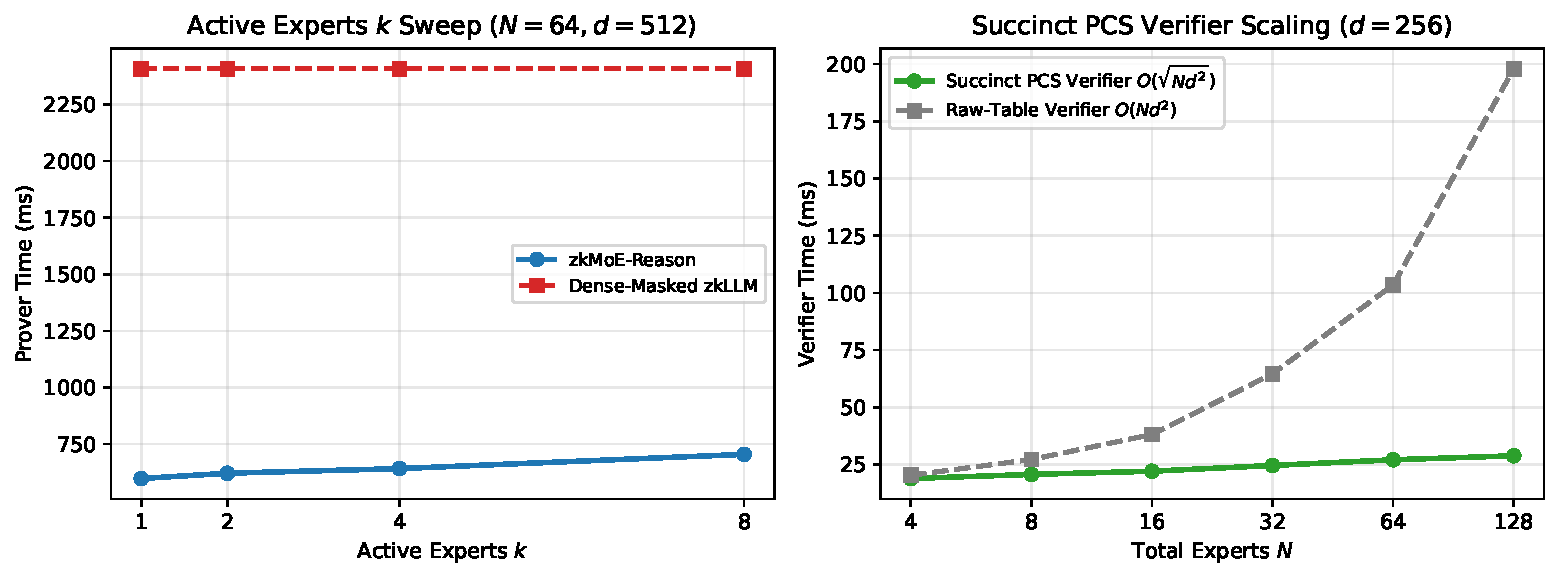
\includegraphics[width=\linewidth]{../results/exp5_ablations.pdf}
    \caption{Left: $k$ sweep at $N=64$, $d=512$. Right: verifier time with the succinct commitment opening versus rereading the raw expert table ($d=256$).}
    \label{fig:exp5}
\end{figure}
At $d=256$ the succinct verifier takes $18.8$, $22.0$, $27.0$ and $28.8$\,ms for $N=4,16,64,128$ with opening sizes $77$--$327$\,KB, while the raw-table verifier takes $20.3$, $38.1$, $103.5$ and $197.9$\,ms. The two are comparable at $N=4$ and the succinct verifier wins from $N\approx8$. The $77$--$327$\,KB opening is large for a single layer, and we have not measured full-model proof sizes. We use a tensor-code commitment with $t=16$ queried columns; we did not compute concrete soundness parameters for the code, so the opening error $\epsilon_{\text{PCS}}$ above is not quantified.

\paragraph{Run-to-run variation.} The same configuration ($N=64$, $d=512$, $k=2$) took $309$\,ms in the scaling run (Table~\ref{tab:exp1}) and $621$\,ms in the $k$ sweep, with dense baselines of $1{,}924$ and $2{,}407$\,ms; the ratio is $6.2\times$ in one run and $3.9\times$ in the other. We did not identify the cause (the runs were separate processes on a shared machine). Ratios in this section should be read as uncertain by roughly a factor of two.

\section{Limitations}
\label{sec:limits}
\begin{itemize}[leftmargin=*,itemsep=2pt]
    \item \textbf{No routing privacy.} See Section~\ref{sec:lookup}. The earlier zero-knowledge and simulator claims are withdrawn.
    \item \textbf{$\Theta(Nd^2)$ prover scan.} The pipeline is not sublinear in $N$; it replaces $N$ sumchecks with one scan.
    \item \textbf{No composition.} The router mask $m$, the lookup indicators $u^{(i)}$, the layer outputs and the visible answer are not bound into one relation or one theorem. Attention, normalization and activation circuits are not proved.
    \item \textbf{Hidden-reasoning folding removed.} The repository contains a prototype folding accumulator for chain-of-thought steps and a mutation test suite that perturbs it. That is a software check that our verifier rejects the perturbations we wrote, not evidence of soundness; we make no claim about it, and the earlier $100\%$ detection table is withdrawn.
    \item \textbf{Own baseline, one machine, synthetic weights, three repetitions.} Medians over three runs on a shared machine carry noise. No comparison with ZK-DeepSeek, VERIF or any external prover was run.
    \item \textbf{Prototype code.} Not audited; field and commitment code have not been checked against test vectors from other implementations.
\end{itemize}

\section{Conclusion}
A prover that proves only the active experts and checks the expert table through one projection and one commitment opening is cheaper than a one-sumcheck-per-expert baseline at the sizes we tested, by a factor that shrinks from $13\times$ to under $3\times$ as $d$ grows, because the projection scan is $\Theta(Nd^2)$. A threshold range relation for top-$k$ is far smaller than a sorting network. Hiding the routing and composing the pieces into a proof of full MoE inference remain open.

\paragraph{Artifact.} Code, raw JSON results and the exact commands are at \url{https://github.com/npow/zkmoe-reason}, tag \texttt{v1}.

\bibliographystyle{plain}
\bibliography{references}

\end{document}
